\documentclass[11pt,a4paper]{article}

\usepackage[margin=1in]{geometry}
\usepackage[T1]{fontenc}
\usepackage[utf8]{inputenc}
\usepackage{lmodern}
\usepackage{microtype}
\usepackage{graphicx}
\usepackage{booktabs}
\usepackage{longtable}
\usepackage{tabularx}
\usepackage{array}
\usepackage{xcolor}
\usepackage{enumitem}
\usepackage{hyperref}
\usepackage{amsmath}
\usepackage{amssymb}
\usepackage{float}

\hypersetup{
  colorlinks=true,
  linkcolor=blue!55!black,
  urlcolor=blue!55!black,
  citecolor=blue!55!black
}

\setlist[itemize]{topsep=2pt,itemsep=2pt,parsep=0pt}
\setlist[enumerate]{topsep=2pt,itemsep=2pt,parsep=0pt}
\renewcommand{\arraystretch}{1.15}

\newcommand{\code}[1]{\texttt{\detokenize{#1}}}
\newcommand{\stage}[1]{\textbf{Stage #1}}
\newcommand{\metric}[1]{\textsc{#1}}
\newcommand{\cootwo}{CO$_2$}

\title{\textbf{Meme Detoxification Project Notes}\\
\large Explain-then-Rewrite: Leveraging Hate Explanation Generation for Targeted Meme Text Detoxification}
\author{Prepared from the repository, poster, training code, inference code, and reported results}
\date{May 26, 2026}

\begin{document}
\maketitle
\tableofcontents
\newpage

\section{Executive Summary}

This project tackles hateful meme moderation as a \textbf{text rewriting} problem rather than a pure detection or censorship problem. A harmful meme can combine an image and a short caption so that the harmful meaning is only visible when both modalities are read together. Instead of removing the meme, the system tries to rewrite the overlaid text into a safer version that preserves the topic, tone, and visual coherence as much as possible.

The central idea is an \textbf{explain-then-rewrite teacher-student pipeline}. A large multimodal model, LLaVA-Next 7B, reads the meme image and text, writes a structured explanation of why the meme is harmful, and then produces a pseudo-detoxified rewrite. Those pseudo-rewrites become supervision for a much smaller BART-large student model. BART is fine-tuned with LoRA so only about 17M parameters are trained out of roughly 400M total parameters. The result is a lightweight student that can run much faster than the LLaVA teacher.

The project evaluates several systems on 280 held-out test memes:

\begin{itemize}
  \item LLaVA-Next teacher pseudo-rewrites, used as an upper-bound reference.
  \item DetoxLLM-7B, a text-only detoxification baseline.
  \item BART-large without fine-tuning, as an internal ablation.
  \item Four LoRA-fine-tuned BART students: \code{full}, \code{target_only}, \code{visual_only}, and \code{none}.
  \item A CLIP Proxy + BART path, where a small MLP predicts BART encoder soft tokens from CLIP image/text embeddings.
\end{itemize}

The main result is that fine-tuned BART improves over DetoxLLM on text non-toxicity while being far cheaper to run. The best student systems reach text STA around 0.95--0.96, compared with 0.94 for DetoxLLM. The proxy path reaches the best semantic similarity and CLIP alignment, but detoxifies less aggressively.

\section{What The Project Is About}

\subsection{Problem}

The project starts from the observation that harmful memes are multimodal. The caption alone may look ambiguous, and the image alone may look harmless, but the combination can target a protected group, stereotype people, or imply hateful meaning. Traditional moderation usually acts after exposure by removing, blurring, or suppressing content. This project proposes a more constructive alternative: \textbf{detoxify the meme text}.

The intended output is not a label such as ``hateful'' or ``not hateful''. It is a rewritten meme caption:

\begin{quote}
Given an image and its original overlaid text, produce a safer text rewrite that removes hateful framing while preserving the meme topic and intended meaning.
\end{quote}

The poster frames this as a shift from censorship to detoxification. The goal is not to defend the original harmful content, but to preserve the communicative intent when possible without retaining the identity-based attack.

\subsection{Research Hypothesis}

The hypothesis is:

\begin{quote}
A large multimodal teacher can explain the harmful image-text interaction and generate safer pseudo-rewrites; then a compact BART-large student can learn this behavior through parameter-efficient fine-tuning.
\end{quote}

This gives the project two related goals:

\begin{itemize}
  \item \textbf{Quality goal:} rewrite hateful meme text so it becomes less toxic while remaining semantically and visually aligned.
  \item \textbf{Deployment goal:} avoid running a 7B vision-language model at inference time whenever possible.
\end{itemize}

\subsection{High-Level Pipeline}

\begin{figure}[H]
  \centering
  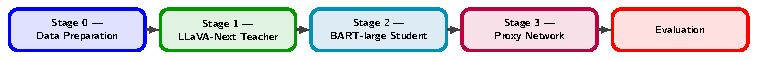
\includegraphics[width=0.95\linewidth]{architecture_diagram.pdf}
  \caption{Project training pipeline, as used in the poster.}
\end{figure}

The pipeline is:

\begin{enumerate}
  \item \textbf{Stage 0:} OCR + CLIP filtering keeps meme-like images with readable text.
  \item \textbf{Unified split builder:} combines HarMeme, MAMI, and MMHS150K into stratified train/validation/test splits.
  \item \textbf{Stage 1:} LLaVA-Next generates structured explanations and pseudo-rewrites, then quality filters the rewrites.
  \item \textbf{Stage 2 dataset builder:} keeps clean pseudo-rewrite pairs and writes \code{train.jsonl}, \code{val.jsonl}, and \code{test.jsonl}.
  \item \textbf{Stage 2 training:} BART-large is fine-tuned with LoRA under several conditioning settings.
  \item \textbf{Proxy training:} a CLIP-to-BART MLP learns to approximate BART encoder memory without LLaVA.
  \item \textbf{Evaluation:} all systems are scored on the same held-out test examples.
\end{enumerate}

\section{Datasets And Data Construction}

\subsection{Source Datasets}

The project uses three meme or image-text hate datasets:

\begin{longtable}{p{0.18\linewidth}p{0.48\linewidth}p{0.24\linewidth}}
\toprule
\textbf{Dataset} & \textbf{Role in project} & \textbf{Labels}\\
\midrule
HarMeme & COVID-19 and US-politics harmful meme collection. Used as one curated meme source. & Harmful vs not harmful.\\
MAMI & Misogynous meme dataset from SemEval 2022. Used as a curated gender/misogyny source. & Misogynous vs not misogynous.\\
MMHS150K & Twitter image-text hate speech collection. Large and noisy, so it needs stricter image filtering. & Majority vote over annotator hate labels.\\
\bottomrule
\end{longtable}

The implementation loaders are in \path{data/preprocess/build_unified_splits.py}. HarMeme and MAMI are already curated meme datasets; MMHS150K is more heterogeneous because it comes from Twitter and contains many plain photos, screenshots, video thumbnails, and UI captures.

\subsection{Stage 0: OCR + CLIP Filtering}

Stage 0 is implemented in \path{data/preprocess/filter_meme_images.py}. It produces a per-dataset \code{manifest.csv} with image path, OCR text, character count, CLIP scores, and a Boolean \code{kept} flag.

The filtering logic is:

\begin{enumerate}
  \item Run EasyOCR on the image.
  \item Keep only images whose extracted text length is between 10 and 300 characters.
  \item Run CLIP ViT-L/14 to decide whether the image looks meme-like.
\end{enumerate}

The CLIP rule is dataset-specific:

\begin{longtable}{p{0.18\linewidth}p{0.25\linewidth}p{0.47\linewidth}}
\toprule
\textbf{Dataset} & \textbf{CLIP setup} & \textbf{Keep rule}\\
\midrule
HarMeme & Binary prompt comparison. & Keep if the meme prompt scores higher than the screenshot prompt.\\
MAMI & Binary prompt comparison. & Same as HarMeme.\\
MMHS150K & Five-way prompt comparison. & Keep only if the meme prompt is the top class and its softmax probability is at least 0.45.\\
\bottomrule
\end{longtable}

The MMHS150K negative prompts represent common false positives: text screenshots, social-media video thumbnails, plain photos, and mobile/social UI screenshots. This stricter rule is necessary because MMHS150K is much noisier than the curated datasets.

\subsection{Unified Splits}

The split builder reads the Stage 0 manifests, keeps only \code{kept=True} examples, and creates 80/10/10 train/validation/test splits. The split is stratified by \code{(dataset, hateful)} so every split contains a proportional mix of datasets and labels.

The output files are:

\begin{itemize}
  \item \code{unified_train.csv}
  \item \code{unified_val.csv}
  \item \code{unified_test.csv}
  \item \code{split_stats.json}
\end{itemize}

\subsection{Stage 2 Dataset Statistics}

After LLaVA pseudo-rewrite generation and filtering, the reported Stage 2 supervision contains:

\begin{longtable}{lr}
\toprule
\textbf{Quantity} & \textbf{Count}\\
\midrule
Loaded LLaVA rewrite rows for train & 7,918\\
Dropped because Stage 1 filters failed & 3,701\\
Dropped because of parse errors & 560\\
Kept after parse/toxicity filtering & 3,657\\
Kept after rewrite text quality filtering & 3,578\\
\textbf{Train examples} & \textbf{3,578}\\
\textbf{Validation examples} & \textbf{269}\\
\textbf{Test examples} & \textbf{280}\\
\bottomrule
\end{longtable}

The important design choice is that the final training set is smaller but cleaner. This is sensible for LoRA fine-tuning because the model updates only a small adapter subspace; noisy supervision would quickly dominate the signal.

\section{Main Model Components}

\subsection{LLaVA-Next Teacher}

The teacher is \code{llava-hf/llava-v1.6-mistral-7b-hf}, wrapped in \path{models/explainer.py}. It is used in Stage 1 for two tasks:

\begin{enumerate}
  \item Generate a structured explanation.
  \item Generate a detoxified pseudo-rewrite using that explanation.
\end{enumerate}

The explanation prompt forces JSON with three fields:

\begin{itemize}
  \item \code{target_group}: one of \code{race_ethnicity}, \code{nationality}, \code{religion}, \code{gender}, \code{sexual_orientation}, \code{disability}, or \code{other}.
  \item \code{visual_evidence}: a short concrete image cue.
  \item \code{implicit_meaning}: one sentence explaining why image plus text is harmful.
\end{itemize}

The rewrite prompt then asks LLaVA to remove slurs, insults, stereotypes, and group-blaming language while keeping the same topic and meme-like style. The output is constrained to one short plain-text rewrite with no markdown, URLs, labels, or explanations.

The implementation includes robust parsing and cleanup:

\begin{itemize}
  \item JSON fence stripping and last-balanced-object extraction.
  \item Target-group normalization.
  \item Fallback defaults for hateful examples whose explanations are null.
  \item Rewrite sanitization to remove markdown, mentions, hashtags, URLs, repeated punctuation, and artifacts.
\end{itemize}

\subsection{BART Student}

The student is \code{facebook/bart-large}. BART is an encoder-decoder sequence-to-sequence model, so the task is naturally represented as:

\begin{quote}
encoder input = original meme text plus optional explanation context; decoder target = LLaVA pseudo-rewrite.
\end{quote}

BART does not directly consume image pixels during standard Stage 2 training. The visual information is distilled into text fields generated by LLaVA, especially \code{visual_evidence} and \code{implicit_meaning}. Images are only used during evaluation metrics.

\subsection{Conditioning Settings}

The intended ablations are:

\begin{longtable}{p{0.22\linewidth}p{0.68\linewidth}}
\toprule
\textbf{Condition} & \textbf{Intended information available to BART}\\
\midrule
\code{full} & Target group, visual evidence, implicit harmful meaning, and original text.\\
\code{target_only} & Target group and original text; visual evidence and implicit meaning set to \code{null}.\\
\code{visual_only} & Visual evidence and original text; target group and implicit meaning set to \code{null}.\\
\code{none} & Only original text; all explanation fields set to \code{null}.\\
\bottomrule
\end{longtable}

The legacy input format is:

\begin{quote}
\code{[T: target] [V: visual_evidence] [M: implicit_meaning] | original_text}
\end{quote}

The explicit detox input format is:

\begin{quote}
\code{Task: rewrite the original meme text to be non-toxic while preserving the meme topic and intended meaning. Context: target group = ...; visual evidence = ...; implicit harmful meaning = ... . Original meme text to detoxify: ...}
\end{quote}

\paragraph{Important implementation caveat.}
The central \code{MemeRewriter.format_input} method in \path{models/rewriter.py} correctly applies condition masking for both \code{legacy} and \code{explicit_detox}. However, the training formatter in \path{training/train_stage2_phase2.py} and the inference formatter in \path{inference/run_stage2.py} compute condition-specific prefixes but, in the \code{explicit_detox} branch, still insert the unmasked \code{target_group}, \code{visual_evidence}, and \code{implicit_meaning}. Therefore, if the reported \code{explicit_detox} run used those scripts, the four named ablations should be interpreted cautiously: the prompts may not have enforced the intended field masking in that format.

\subsection{LoRA Adaptation}

Stage 2 uses LoRA rather than full fine-tuning. The base BART weights are frozen and low-rank trainable matrices are added to selected modules:

\[
W' = W + \frac{\alpha}{r}BA
\]

where \(W\) is the frozen original weight, \(A\) and \(B\) are trainable low-rank matrices, \(r=32\), and \(\alpha=64\).

The target modules are:

\begin{itemize}
  \item attention projections: \code{q_proj}, \code{k_proj}, \code{v_proj}, \code{out_proj}
  \item feed-forward projections: \code{fc1}, \code{fc2}
\end{itemize}

\begin{figure}[H]
  \centering
  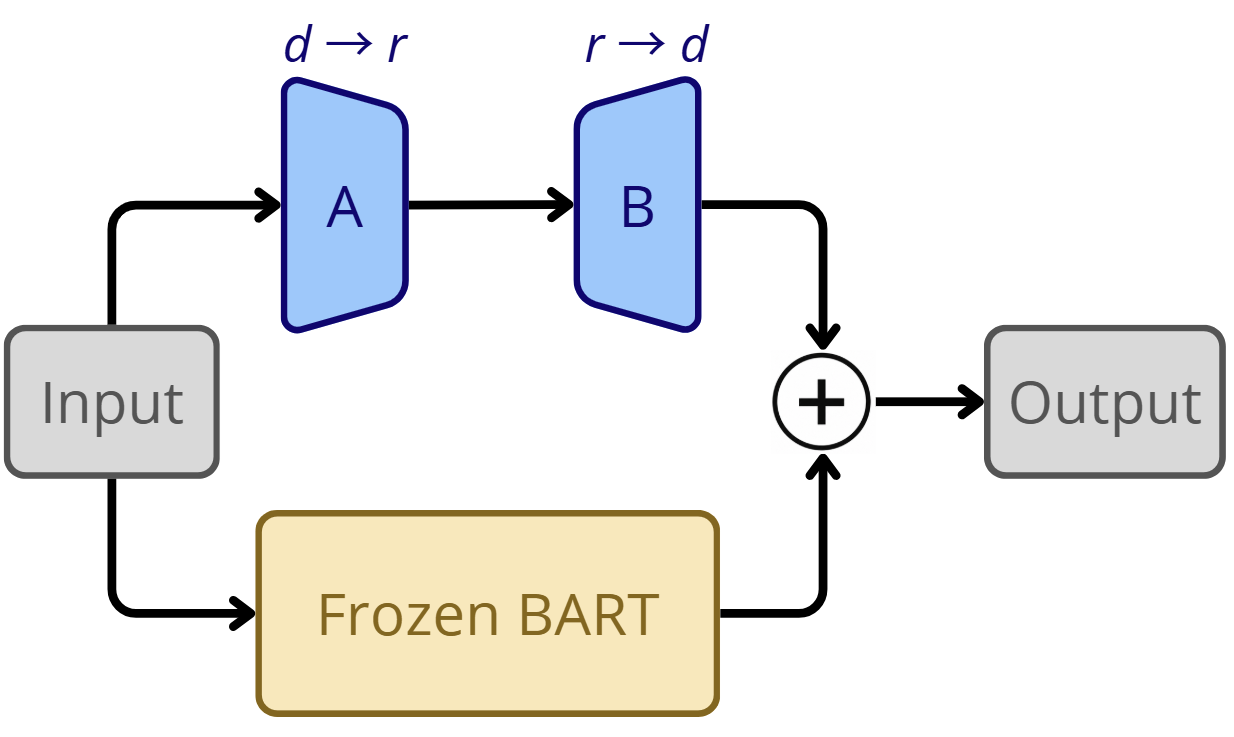
\includegraphics[width=0.7\linewidth]{lora.png}
  \caption{LoRA idea used for parameter-efficient adaptation.}
\end{figure}

The reported configuration trains about 17M parameters out of roughly 400M, about 4.3 percent.

\subsection{CLIP Proxy}

The proxy model is in \path{models/proxy.py} and \path{training/train_proxy.py}. It is a deployment experiment: can the system avoid LLaVA at inference time while still giving BART some multimodal context?

The proxy input is:

\[
\text{concat}(\text{CLIP image embedding}, \text{CLIP text embedding}) \in \mathbb{R}^{1536}
\]

because CLIP ViT-L/14 gives 768-dimensional image embeddings and 768-dimensional text embeddings.

The proxy network is a three-layer MLP:

\[
1536 \rightarrow 1024 \rightarrow 1024 \rightarrow K \times 1024
\]

where \(K=16\) by default. The output is a short sequence of predicted BART encoder soft tokens. During training, the target is the full-condition BART encoder memory, pooled to \(K\) tokens. The proxy is trained with MSE loss.

\section{Stage 1: Pseudo-Label Generation In Detail}

Stage 1 is implemented in \path{inference/run_stage1_sharded.py}. It runs after Stage 0 and unified split construction.

\subsection{Input Selection}

The script reads a split CSV such as \code{unified_train.csv}. It filters to Stage-0-kept images, optionally keeps only hateful examples, and then shards the records by:

\[
\text{row index} \bmod \text{num shards} = \text{shard id}
\]

The cluster workflow uses 8 shards for train and 2 shards each for validation and test.

\subsection{Explanation Pass}

For each selected meme:

\begin{enumerate}
  \item Load the image.
  \item Read the meme text from the split row.
  \item Ask LLaVA for a structured JSON explanation.
  \item Parse and normalize the JSON.
  \item If the example is hateful and fields are missing, fill safe defaults so BART always receives non-empty context.
\end{enumerate}

The explanation records are saved to shard JSONL files.

\subsection{Rewrite Pass}

Only hateful examples receive pseudo-rewrites. LLaVA is prompted with the image, original text, and structured explanation. The code allows multiple rewrite attempts. Each candidate is sanitized and rejected if it has obvious format problems:

\begin{itemize}
  \item empty output,
  \item too short or too long,
  \item URL, domain, hashtag, or mention,
  \item symbol-heavy output,
  \item repeated tokens or low lexical diversity,
  \item exact copy of the original,
  \item optional near-copy rejection using lexical or character similarity thresholds.
\end{itemize}

\subsection{Quality Filtering}

For valid rewrite candidates, Stage 1 computes:

\begin{itemize}
  \item \textbf{text toxicity} with \code{s-nlp/roberta_toxicity_classifier};
  \item \textbf{text STA}, defined here as \(1 - P(\text{toxic})\);
  \item \textbf{toxicity drop}, original toxicity minus rewrite toxicity;
  \item \textbf{BERTScore F1} between original and rewrite;
  \item \textbf{VisualBERT multimodal toxicity}, stored as annotation/evaluation information.
\end{itemize}

A rewrite passes if:

\begin{itemize}
  \item text STA is above the threshold,
  \item BERTScore is above the minimum threshold,
  \item toxicity drop is non-negative or above the configured minimum when the source is sufficiently toxic.
\end{itemize}

The script writes all records, both passed and failed, with a \code{passed_stage1_filters} flag. This is important because the Stage 2 dataset builder later makes the final supervision decision.

\section{Stage 2 Dataset Builder In Detail}

The dataset builder is \path{data/preprocess/build_stage2_dataset.py}. It reads merged Stage 1 rewrite JSONL files and creates the files consumed by BART training.

\subsection{Filtering Rules}

Rows are kept only if:

\begin{enumerate}
  \item there was no explanation parse error;
  \item \code{passed_stage1_filters} is true, unless explicitly overridden;
  \item \code{toxicity_drop > min_toxicity_drop}, with default \code{min_toxicity_drop = 0.0};
  \item the sanitized rewrite passes additional text-quality checks;
  \item the rewrite is not identical to the source;
  \item optional source similarity is below \code{max_source_similarity}; the RunAI script uses 0.95.
\end{enumerate}

\subsection{Record Format}

Each final Stage 2 record stores:

\begin{itemize}
  \item \code{id}
  \item \code{image_path}
  \item \code{original_text}
  \item \code{target_group}
  \item \code{visual_evidence}
  \item \code{implicit_meaning}
  \item \code{input_text}
  \item \code{target_text}, the pseudo-rewrite
  \item Stage 1 metadata such as STA, BERTScore, toxicity drop, and source similarity
\end{itemize}

When validation and test Stage 1 rewrite files are provided, the builder uses proper held-out splits rather than randomly splitting the training file. This is the current intended setup.

\section{Stage 2 BART Training In Detail}

\subsection{Current Training Setup}

The main current training script is \path{training/train_stage2_phase2.py}. The README states that the current reported pipeline starts directly from \code{facebook/bart-large}; Phase 1 ParaDetox warm-up exists in \path{training/train_stage2_phase1.py} but is kept for reference rather than used in the current run.

The reported Phase 2 setup is:

\begin{longtable}{p{0.34\linewidth}p{0.56\linewidth}}
\toprule
\textbf{Item} & \textbf{Value}\\
\midrule
Base model & \code{facebook/bart-large}\\
Training data & Meme pseudo-rewrites from Stage 1 only\\
Train/val/test & 3,578 / 269 / 280 examples\\
Epochs & 5\\
Batch size & 8\\
Learning rate & \(1 \times 10^{-4}\) in the RunAI script\\
Warmup & 50 steps in the RunAI script\\
Weight decay & 0.01\\
Precision & bf16 if supported, otherwise fp16 on GPU\\
Generation & beam search with 4 beams, max length 64, no-repeat n-gram constraints\\
LoRA & \(r=32\), \(\alpha=64\), dropout 0.05\\
Seed & 42\\
\bottomrule
\end{longtable}

\subsection{Training Data Flow}

For each example, the dataset class builds a condition-specific encoder input and tokenizes both input and target:

\begin{enumerate}
  \item \code{format_input(...)} builds the prompt.
  \item BART tokenizer encodes the prompt, truncating to 128 tokens.
  \item BART tokenizer encodes \code{target_text}, also truncating to 128 tokens.
  \item \code{DataCollatorForSeq2Seq} dynamically pads the batch and masks label padding with \(-100\).
\end{enumerate}

The model learns by standard sequence-to-sequence teacher forcing: predict the pseudo-rewrite token sequence conditioned on the prompt.

\subsection{Generation Configuration}

The training script resets BART generation settings before training. This matters because BART checkpoints can inherit summarization-oriented settings that are poor for short detoxification rewrites. The current settings include:

\begin{itemize}
  \item \code{num_beams = 4}
  \item \code{early_stopping = True}
  \item \code{no_repeat_ngram_size = 3}
  \item \code{encoder_no_repeat_ngram_size = 3}
  \item \code{max_length = 64}
  \item \code{min_length = 8} or \code{min_new_tokens = 8} when supported
\end{itemize}

Before training starts, the script runs a pre-training generation sanity check on one validation example. This catches degenerate generation settings early.

\subsection{Metrics During Training}

Every evaluation checkpoint computes:

\begin{itemize}
  \item \textbf{ROUGE-1/2/L}: overlap with the LLaVA pseudo-rewrite target.
  \item \textbf{Collapse rate}: fraction of empty, one-token, or highly repetitive outputs.
  \item \textbf{Text STA}: fraction of outputs whose toxicity probability is below 0.5.
  \item \textbf{Text toxicity drop}: original text toxicity minus generated text toxicity.
  \item \textbf{Source similarity}: normalized character similarity between original and generated output.
  \item \textbf{Exact and high copy rates}: checks whether the model is copying too much.
  \item \textbf{Detox quality}: a selection score
  \[
  \text{toxicity drop} + 0.10 \cdot \text{ROUGE-L} - 0.25 \cdot \text{high copy rate}.
  \]
  \item \textbf{VisualBERT metrics}: multimodal hate probability and multimodal STA, used only for evaluation.
\end{itemize}

The training logs also print five qualitative examples at every evaluation step:

\begin{quote}
original \(\rightarrow\) generated \(\rightarrow\) reference
\end{quote}

This is useful because the numeric metrics can disagree. For example, a model can get high STA by producing generic safe text, but that may destroy meaning.

\subsection{Checkpoint Export}

PEFT compatibility prevents simply using Hugging Face's automatic best-model loading in the usual way. Instead, the script:

\begin{enumerate}
  \item trains the LoRA model;
  \item searches the logged evaluation entries for the best \code{eval_detox_quality};
  \item loads the corresponding checkpoint adapter if present;
  \item saves the best adapter to \code{lora_adapter};
  \item saves the final-step adapter to \code{lora_adapter_final};
  \item merges the exported adapter into the base BART model;
  \item saves the merged model in the output directory so downstream scripts can load it with \code{BartForConditionalGeneration.from_pretrained}.
\end{enumerate}

The script also writes \code{training_history.json}, including run config, LoRA config, hardware, best metric, and full log history.

\subsection{Training Behavior}

The README reports that training behaves as expected:

\begin{itemize}
  \item training loss decreases for every condition;
  \item validation text STA increases;
  \item text toxicity drop improves;
  \item ROUGE stays stable instead of collapsing;
  \item copy rate is monitored;
  \item VisualBERT STA stays flat at 0, which makes that metric unreliable as an absolute pass/fail signal.
\end{itemize}

For the \code{full} condition, validation loss was:

\begin{longtable}{rr}
\toprule
\textbf{Step} & \textbf{Validation loss}\\
\midrule
200 & 1.4025\\
800 & 1.2254\\
1600 & 1.1890\\
2240 & 1.1948\\
\bottomrule
\end{longtable}

This indicates useful learning through training, with the best reported loss around step 1600.

\begin{figure}[H]
  \centering
  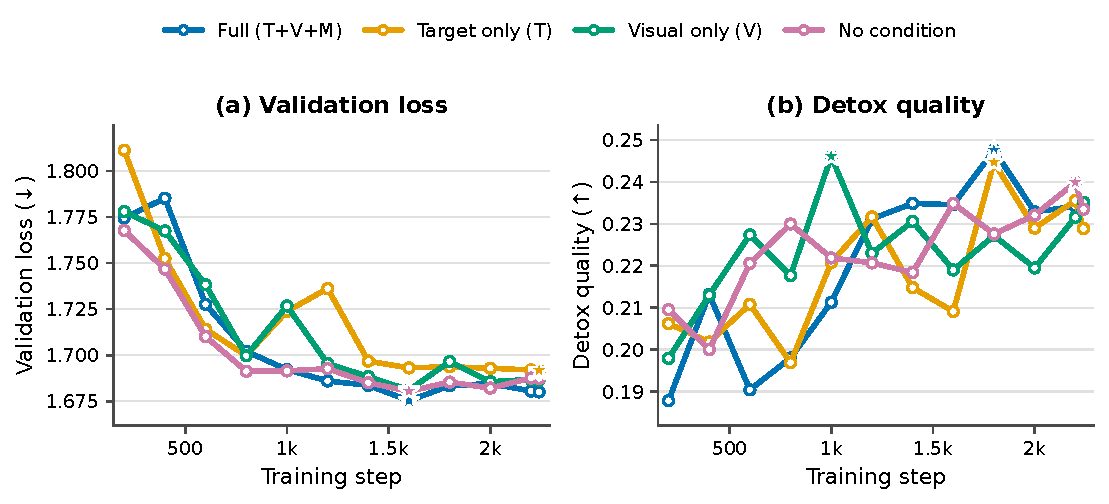
\includegraphics[width=0.82\linewidth]{hmr_training_plots_explicit_detox/phase2_validation_loss_detox_quality_publication.pdf}
  \caption{Validation-loss and detox-quality plot included with the repository.}
\end{figure}

\section{Proxy Training In Detail}

The proxy is trained after the full-condition BART model exists. It does not learn to generate text directly. It learns to predict the encoder-memory representation that BART would have produced from a full explanation prompt.

\subsection{Training Targets}

For each Stage 2 example:

\begin{enumerate}
  \item The frozen full-condition BART encoder processes the original text plus explanation fields.
  \item Its variable-length encoder hidden states are adaptively average-pooled to \(K\) soft tokens.
  \item CLIP encodes the image and original text.
  \item The proxy MLP maps the concatenated CLIP features to the pooled BART encoder soft tokens.
  \item MSE loss trains the proxy to match those soft tokens.
\end{enumerate}

\subsection{Why This Is Interesting}

This is not the same as asking CLIP to generate text. The proxy only produces a continuous hidden-state prefix. The actual language generation is still done by the fine-tuned BART decoder. This means the proxy tries to inject multimodal context into BART without running LLaVA.

\section{Inference Pipeline In Detail}

\begin{figure}[H]
  \centering
  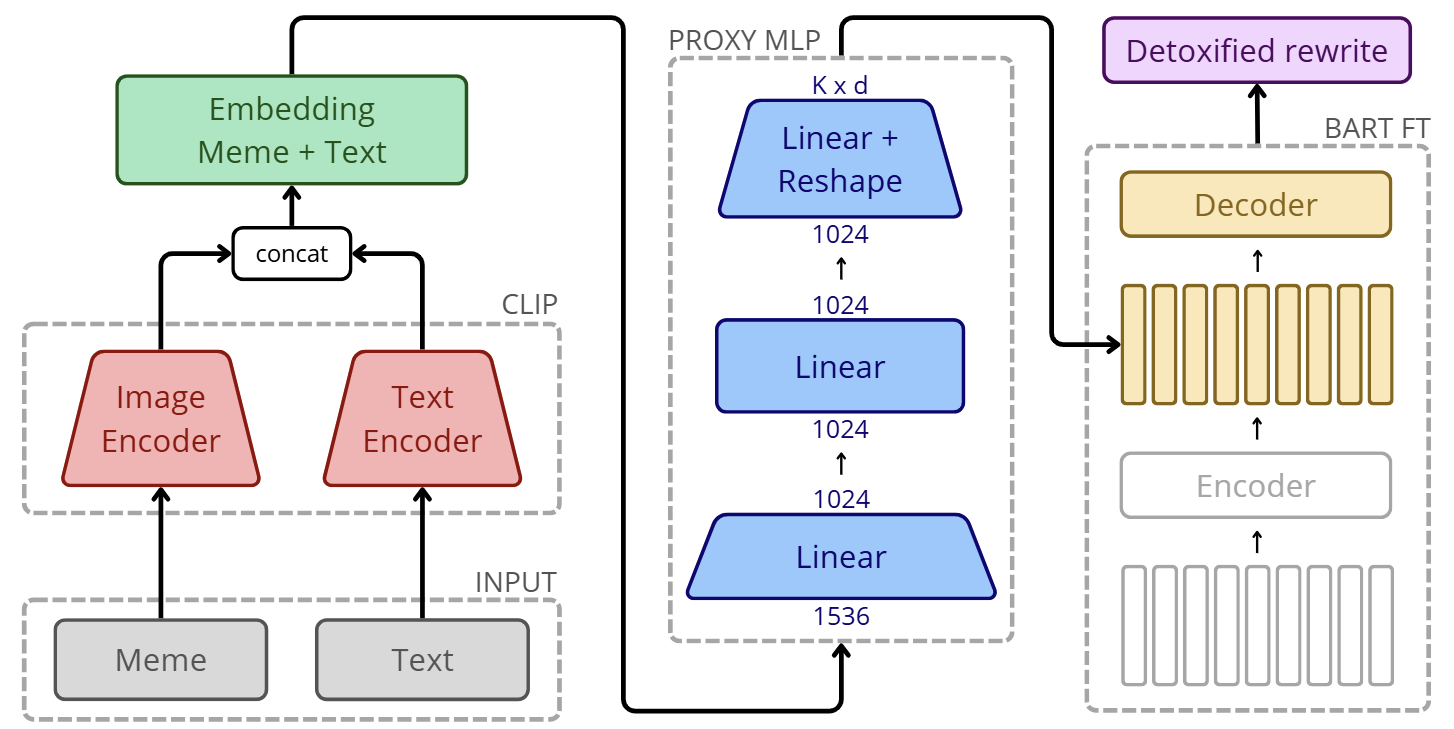
\includegraphics[width=0.95\linewidth]{inference.png}
  \caption{Inference diagram included with the repository.}
\end{figure}

\subsection{Standard BART Inference}

Standard BART inference is implemented in \path{inference/run_stage2.py}.

The script:

\begin{enumerate}
  \item loads \code{test.jsonl} or another Stage 2 JSONL file;
  \item loads either base BART or a merged fine-tuned checkpoint;
  \item builds a condition prompt for each example;
  \item batches prompts;
  \item calls BART generation with beam search and no-repeat n-gram constraints;
  \item writes \code{stage2_rewrites_<condition>.jsonl}.
\end{enumerate}

The output record contains the id, image path, original text, target pseudo-rewrite, generated rewrite, explanation fields, and condition.

\subsection{Proxy + BART Inference}

Proxy inference is implemented in \path{inference/run_proxy_pipeline.py}. It is the VLM-free inference path:

\begin{enumerate}
  \item CLIP encodes the image and original text.
  \item The proxy predicts \(K\) BART encoder soft tokens.
  \item BART also encodes a \code{none} prompt containing the original text.
  \item The proxy tokens are concatenated before the text encoder states.
  \item BART decodes a rewrite from this combined encoder memory.
\end{enumerate}

The key deployment point is that this path uses CLIP + proxy + BART, not LLaVA.

\subsection{Evaluation Pipeline}

The unified evaluation job in \path{scripts/run_evaluate_all_job.sh} runs:

\begin{itemize}
  \item BART base inference for all four conditions;
  \item fine-tuned BART inference for all four conditions;
  \item DetoxLLM inference;
  \item Proxy + BART inference;
  \item \path{evaluation/evaluate.py} once over all collected outputs.
\end{itemize}

Evaluation aligns systems by validation/test ids and computes:

\begin{itemize}
  \item text STA on originals and rewrites;
  \item text STA delta;
  \item BERTScore similarity between original and rewrite;
  \item CLIPScore between image and rewrite;
  \item VisualBERT multimodal hate probability;
  \item VisualBERT multimodal STA;
  \item VisualBERT hate drop.
\end{itemize}

One important implementation detail: evaluation does not sanitize or edit generated rewrites before scoring. The only truncation is internal to CLIPScore because CLIP has a hard 77-token text limit.

\section{Results}

\subsection{Main Test Results}

All main systems were evaluated on the same 280 held-out test examples. The compact results from the README and poster are:

\begingroup
\small
\setlength{\tabcolsep}{3pt}
\begin{longtable}{p{0.30\linewidth}rrrrrrrr}
\toprule
\textbf{System} & \textbf{n} & \textbf{Text STA} & \textbf{Delta} & \textbf{SIM} & \textbf{CLIP} & \textbf{VB hate} & \textbf{VB STA} & \textbf{VB drop}\\
\midrule
\code{llava_teacher} & 280 & 0.9903 & 0.2342 & 0.4722 & 0.6357 & 0.6511 & 0.0000 & -0.0053\\
\code{detoxllm} & 280 & 0.9400 & 0.1839 & 0.4433 & 0.6337 & 0.6489 & 0.0000 & -0.0031\\
\code{bart_finetuned_full} & 280 & 0.9588 & 0.2027 & 0.3395 & 0.6280 & 0.6505 & 0.0000 & -0.0047\\
\code{bart_finetuned_target_only} & 280 & 0.9643 & 0.2082 & 0.3422 & 0.6282 & 0.6518 & 0.0000 & -0.0060\\
\code{bart_finetuned_visual_only} & 280 & 0.9502 & 0.1941 & 0.3301 & 0.6288 & 0.6521 & 0.0000 & -0.0063\\
\code{bart_finetuned_none} & 280 & 0.9508 & 0.1947 & 0.3308 & 0.6287 & 0.6512 & 0.0000 & -0.0054\\
\code{clip_proxy_bart_full} & 280 & 0.8787 & 0.1225 & 0.6004 & 0.6395 & 0.6488 & 0.0000 & -0.0030\\
\bottomrule
\end{longtable}
\endgroup

\subsection{How To Read The Metrics}

\begin{itemize}
  \item \textbf{Text STA} is the mean non-toxic probability from a RoBERTa toxicity classifier. Higher is better.
  \item \textbf{Text STA delta} is rewrite STA minus original STA. Positive means the rewrite is less toxic.
  \item \textbf{SIM} is BERTScore F1 between original and rewrite. Higher means more semantic preservation, but copying can inflate it.
  \item \textbf{CLIP} is image-text alignment between the image and rewrite. Higher means the rewrite still matches the visual content.
  \item \textbf{VisualBERT hate probability and STA} are multimodal evaluation signals, but in this run VisualBERT STA is 0 for every system, so it should not be the main conclusion.
\end{itemize}

\subsection{Main Findings}

\paragraph{LLaVA teacher is the upper-bound reference.}
It has the best text STA and toxicity drop. That is expected because it is both the large multimodal teacher and the source of the pseudo-labels.

\paragraph{Fine-tuned BART beats DetoxLLM on text detoxification.}
The full BART student reaches text STA 0.9588 and toxicity delta 0.2027, compared with DetoxLLM at 0.9400 and 0.1839. The target-only run is slightly higher on these text toxicity metrics. This supports the claim that meme-specific pseudo-supervision helps even when the student is text-only at inference time.

\paragraph{DetoxLLM has higher SIM than fine-tuned BART.}
DetoxLLM reaches SIM 0.4433 while fine-tuned BART is around 0.33--0.34. The README notes that this may partly reflect copying behavior: if a model copies toxic input, BERTScore can look good even though detoxification is weak.

\paragraph{Base BART is not a real baseline for quality.}
Base BART can look highly non-toxic, but its SIM is negative in the reported table. This means it produces text that is safe but semantically disconnected. Fine-tuning moves SIM from about \(-0.061\) to about 0.33--0.34.

\paragraph{Proxy + BART optimizes fidelity more than detoxification.}
The proxy reaches the best SIM, 0.6004, and best CLIPScore, 0.6395, but lower text STA, 0.8787. It is closer to the original and more visually aligned, but less aggressive at removing toxicity.

\paragraph{VisualBERT is not reliable as an absolute pass/fail score here.}
VisualBERT STA is 0 for every system, including the LLaVA teacher. The safest interpretation is that the text metrics show detoxification, SIM/CLIP show preservation/alignment, and VisualBERT is only a weak directional diagnostic in this setup.

\subsection{Qualitative Example}

The poster example rewrites:

\begin{quote}
Optimist: it's half full\\
Pessimist: it's half empty\\
Feminist: it raped me
\end{quote}

into:

\begin{quote}
Optimist: it's half full\\
Pessimist: it's half empty\\
Feminist: it's half full, half empty
\end{quote}

The important point is that the rewrite preserves the three-line glass joke structure while removing the sexual-violence framing.

\section{Compute, Emissions, And Efficiency}

\subsection{Pipeline Carbon Summary}

The README reports the following measured or aggregated \cootwo{} summary on EPFL RCP A100-SXM4-40GB hardware, with Swiss-grid carbon intensity around 34.84 g \cootwo{}/kWh:

\begin{longtable}{p{0.50\linewidth}rrr}
\toprule
\textbf{Stage} & \textbf{GPU time} & \textbf{Energy} & \textbf{\cootwo{}}\\
\midrule
Stage 0 OCR + CLIP filtering, 163,544 images & 2.8 h & 0.76 kWh & 26.7 g\\
Stage 1 LLaVA train shards & 14.1 h & 6.61 kWh & 230.3 g\\
Stage 1 LLaVA val+test shards & 3.5 h & 1.65 kWh & 57.5 g\\
Stage 2 BART LoRA training, 4 conditions & 2.1 h & 0.82 kWh & 28.4 g\\
Stage 3 BART-base inference, 4 conditions & 52.9 min & 0.18 kWh & 6.3 g\\
Stage 3 BART-finetuned inference, 4 conditions & 12.3 min & 0.04 kWh & 1.5 g\\
Proxy inference & 3.4 min & 0.01 kWh & 0.5 g\\
DetoxLLM baseline & 7.9 min & 0.04 kWh & 1.3 g\\
\textbf{Total} & \textbf{about 38 h} & \textbf{10.11 kWh} & \textbf{about 352 g}\\
\bottomrule
\end{longtable}

The key observation is that Stage 1 dominates: more than 80 percent of total pipeline \cootwo{} comes from LLaVA inference. This supports the design choice of paying the teacher cost once during dataset construction, then deploying a smaller student.

\subsection{Single-Inference Benchmark}

The README reports:

\begin{longtable}{lrrrrr}
\toprule
\textbf{System} & \textbf{Params} & \textbf{Load time} & \textbf{Mean inf.} & \textbf{\cootwo{}/inf.} & \textbf{\cootwo{}/280}\\
\midrule
\code{llava_teacher} & 7.6B & 16.8 s & 9,376 ms & 34,340 \(\mu\)g & 9,615 mg\\
\code{detoxllm} & 6.7B & 21.4 s & 1,989 ms & 5,646 \(\mu\)g & 1,581 mg\\
\code{bart_finetuned} & 406M & 4.0 s & 122 ms & 360 \(\mu\)g & 101 mg\\
\bottomrule
\end{longtable}

Pure fine-tuned BART is about 76.6 times faster than LLaVA and 16.3 times faster than DetoxLLM in this benchmark. The poster separately reports CLIP + Proxy + BART FT full at 0.729 s/image, which is 12.9 times faster than LLaVA and 2.7 times faster than DetoxLLM. The difference is that the proxy path includes CLIP and proxy computation, while the pure BART benchmark times the BART text rewrite path.

\section{Limitations And Caveats}

\begin{itemize}
  \item \textbf{Pseudo-label dependence:} the student learns from LLaVA-generated targets, not human-written detoxification references.
  \item \textbf{Dataset noise:} MMHS150K is heterogeneous, and filtering can only partially remove non-meme or low-quality examples.
  \item \textbf{Small final training set:} filtering improves precision but reduces supervision to 3,578 train examples.
  \item \textbf{BART visual grounding is indirect:} standard BART inference sees only text fields, not pixels.
  \item \textbf{VisualBERT metric weakness:} VisualBERT STA is 0 for every system, so it is not a reliable absolute detoxification score here.
  \item \textbf{Ablation interpretation caveat:} the \code{explicit_detox} formatter in the main training/inference scripts appears not to mask fields by condition, so condition comparisons in that format should be treated carefully.
  \item \textbf{Semantic similarity can be misleading:} copying the original can inflate BERTScore even if toxicity remains.
  \item \textbf{Deployment gap:} rewriting overlaid text in real images would still require OCR localization and image editing/inpainting, which are outside this pipeline.
\end{itemize}

\section{What You Need To Know For Questions}

\subsection{Why Not Just Use LLaVA?}

LLaVA is strongest but expensive. It runs two large multimodal generation passes per meme in Stage 1: one for explanation and one for rewrite. The project uses it as a teacher to generate supervision, then distills the behavior into cheaper BART models.

\subsection{Why Use Explanations?}

The explanation fields are a bridge between image understanding and text generation. They convert visual multimodal evidence into textual control signals that BART can consume. This lets BART benefit from multimodal reasoning even though it is a text model.

\subsection{Why Use LoRA?}

The dataset is small, and full BART fine-tuning would update hundreds of millions of parameters. LoRA adapts a small set of low-rank matrices, reducing memory and overfitting risk while preserving the pretrained model.

\subsection{Why Does Base BART Have High STA?}

Because generic or irrelevant text can be non-toxic. High STA alone is not enough. A useful detoxifier must also preserve the meaning and remain image-aligned.

\subsection{Why Is Proxy SIM So High But STA Lower?}

The proxy learns continuous encoder context from CLIP image/text features. It appears to preserve source semantics and image alignment well, but it under-detoxifies compared with the teacher and fine-tuned BART. This is the fidelity-detoxification trade-off.

\section{Three-Minute Presentation Script}

\subsection*{Minute 1: Introduction, Dataset, And Preprocessing}

\textbf{0--20 seconds.}
``Our project is about harmful meme detoxification. Most moderation systems treat hateful memes as a detection or censorship problem: classify the meme, then remove it or blur it. We take a different approach. We try to rewrite the meme text so it becomes non-toxic while preserving the original topic, meme structure, and visual coherence.''

\textbf{20--40 seconds.}
``The challenge is that memes are multimodal. The caption alone can look ambiguous, and the image alone can look harmless, but together they can create an identity-based attack or stereotype. So we need a system that understands the image-text interaction, not just the text.''

\textbf{40--60 seconds.}
``We use three datasets: HarMeme, MAMI, and MMHS150K. Before training, we run Stage 0 preprocessing. EasyOCR extracts overlaid text, and we keep images with 10 to 300 OCR characters. Then CLIP filters out non-meme-like images. HarMeme and MAMI use a binary meme-versus-screenshot CLIP check, while MMHS150K uses a stricter five-prompt filter because it contains many noisy Twitter images such as plain photos, screenshots, and video thumbnails.''

\subsection*{Minute 2: Training And Inference Pipeline}

\textbf{60--80 seconds.}
``After preprocessing, we build stratified train, validation, and test splits across the three datasets. Then Stage 1 uses LLaVA-Next as a multimodal teacher. For each hateful meme, LLaVA first generates a structured explanation with three fields: target group, visual evidence, and implicit harmful meaning.''

\textbf{80--105 seconds.}
``LLaVA then uses that explanation to generate a pseudo-detoxified rewrite. These pseudo-rewrites are filtered using parsing checks, rewrite quality checks, text toxicity reduction from a RoBERTa toxicity classifier, and BERTScore similarity. The goal is to keep rewrites that are safer but still semantically related to the original meme.''

\textbf{105--135 seconds.}
``Stage 2 trains BART-large as the student model. The encoder input is the original meme text plus optional explanation context, and the target text is the LLaVA pseudo-rewrite. BART is trained with standard sequence-to-sequence cross-entropy loss: at each decoder step, it predicts the next target token given the encoder input and previous target tokens. We fine-tune with LoRA, so most BART weights stay frozen and only low-rank adapter matrices are updated, about 17 million trainable parameters out of roughly 400 million.''

\textbf{135--160 seconds.}
``At inference, the fine-tuned BART model can rewrite meme text directly from the formatted prompt, without running LLaVA. We also test a CLIP Proxy plus BART path: CLIP encodes the image and text, a small MLP predicts BART encoder soft tokens, and BART decodes the rewrite. This explores a VLM-free deployment path that still injects some multimodal information.''

\subsection*{Minute 3: Validation, Limitations, And Conclusions}

\textbf{160--180 seconds.}
``We evaluate on 280 held-out test memes. The main metrics are text STA, which measures non-toxic probability, text STA delta, BERTScore similarity, CLIPScore image-text alignment, and VisualBERT multimodal toxicity. The LLaVA teacher is the strongest upper-bound reference, with text STA about 0.990.''

\textbf{180--205 seconds.}
``Our fine-tuned BART models reach text STA around 0.95 to 0.96, improving over the DetoxLLM baseline at 0.94. The full BART model reaches 0.959 text STA and 0.203 toxicity reduction. The proxy model gets the best semantic similarity and CLIPScore, but lower detoxification, which shows a fidelity-versus-detoxification trade-off.''

\textbf{205--225 seconds.}
``There are important limitations. The student depends on LLaVA pseudo-labels, so teacher errors can propagate. The final filtered dataset is relatively small. BART does not directly see pixels in the standard inference path; image information is distilled through text explanations. Also, VisualBERT STA is zero for all systems, so we treat that metric cautiously rather than as a reliable absolute pass/fail score.''

\textbf{225--240 seconds.}
``Overall, the project shows that multimodal explanations from a large teacher can be distilled into a much lighter BART student for meme text detoxification. The student does not beat LLaVA, but it is far cheaper and improves over a text-only detoxification baseline on toxicity reduction. The next steps would be better human-quality rewrite data, stronger multimodal evaluation, and eventually OCR plus inpainting so rewritten text can be inserted back into real meme images.''

\section{Code Map}

\begin{longtable}{p{0.32\linewidth}p{0.58\linewidth}}
\toprule
\textbf{File} & \textbf{What it does}\\
\midrule
\path{poster_template_DL/poster.tex} & Final poster text, reported results, qualitative example, limitations, and conclusion.\\
\path{README.md} & Most complete project description, workflow, current experiment report, results, and emissions.\\
\path{data/preprocess/filter_meme_images.py} & Stage 0 EasyOCR + CLIP filtering.\\
\path{data/preprocess/build_unified_splits.py} & Loads all datasets and creates stratified train/val/test CSVs.\\
\path{inference/run_stage1_sharded.py} & LLaVA explanations, pseudo-rewrites, scoring, filtering, sharding, and emissions.\\
\path{models/explainer.py} & LLaVA wrapper, prompts, parsing, normalization, batch explain/rewrite.\\
\path{data/preprocess/build_stage2_dataset.py} & Converts Stage 1 rewrite outputs into BART train/val/test JSONL files.\\
\path{training/train_stage2_phase2.py} & Main BART LoRA fine-tuning script.\\
\path{models/rewriter.py} & BART inference wrapper and condition formatting.\\
\path{inference/run_stage2.py} & BART inference over a Stage 2 split.\\
\path{models/proxy.py} & CLIP-to-BART soft-token proxy network and trainer helper.\\
\path{training/train_proxy.py} & Proxy training entry point.\\
\path{inference/run_proxy_pipeline.py} & Proxy + BART inference path.\\
\path{evaluation/evaluate.py} & Loads all system outputs and writes final evaluation summaries.\\
\path{evaluation/metrics.py} & Text STA, BERTScore SIM, CLIPScore, and VisualBERT metrics.\\
\path{baselines/run_detoxllm_baseline.py} & DetoxLLM text-only baseline.\\
\bottomrule
\end{longtable}

\end{document}
